\documentclass[twoside]{book}

% Packages required by doxygen
\usepackage{calc}
\usepackage{doxygen}
\usepackage{graphicx}
\usepackage[utf8]{inputenc}
\usepackage{makeidx}
\usepackage{multicol}
\usepackage{multirow}
\usepackage{textcomp}
\usepackage[table]{xcolor}

% Font selection
\usepackage[T1]{fontenc}
\usepackage{mathptmx}
\usepackage[scaled=.90]{helvet}
\usepackage{courier}
\usepackage{amssymb}
\usepackage{sectsty}
\renewcommand{\familydefault}{\sfdefault}
\allsectionsfont{%
  \fontseries{bc}\selectfont%
  \color{darkgray}%
}
\renewcommand{\DoxyLabelFont}{%
  \fontseries{bc}\selectfont%
  \color{darkgray}%
}

% Page & text layout
\usepackage{geometry}
\geometry{%
  a4paper,%
  top=2.5cm,%
  bottom=2.5cm,%
  left=2.5cm,%
  right=2.5cm%
}
\tolerance=750
\hfuzz=15pt
\hbadness=750
\setlength{\emergencystretch}{15pt}
\setlength{\parindent}{0cm}
\setlength{\parskip}{0.2cm}
\makeatletter
\renewcommand{\paragraph}{%
  \@startsection{paragraph}{4}{0ex}{-1.0ex}{1.0ex}{%
    \normalfont\normalsize\bfseries\SS@parafont%
  }%
}
\renewcommand{\subparagraph}{%
  \@startsection{subparagraph}{5}{0ex}{-1.0ex}{1.0ex}{%
    \normalfont\normalsize\bfseries\SS@subparafont%
  }%
}
\makeatother

% Headers & footers
\usepackage{fancyhdr}
\pagestyle{fancyplain}
\fancyhead[LE]{\fancyplain{}{\bfseries\thepage}}
\fancyhead[CE]{\fancyplain{}{}}
\fancyhead[RE]{\fancyplain{}{\bfseries\leftmark}}
\fancyhead[LO]{\fancyplain{}{\bfseries\rightmark}}
\fancyhead[CO]{\fancyplain{}{}}
\fancyhead[RO]{\fancyplain{}{\bfseries\thepage}}
\fancyfoot[LE]{\fancyplain{}{}}
\fancyfoot[CE]{\fancyplain{}{}}
\fancyfoot[RE]{\fancyplain{}{\bfseries\scriptsize Generated on Mon Feb 13 2017 14\-:04\-:13 for Omni\-\_\-\-Driver by Doxygen }}
\fancyfoot[LO]{\fancyplain{}{\bfseries\scriptsize Generated on Mon Feb 13 2017 14\-:04\-:13 for Omni\-\_\-\-Driver by Doxygen }}
\fancyfoot[CO]{\fancyplain{}{}}
\fancyfoot[RO]{\fancyplain{}{}}
\renewcommand{\footrulewidth}{0.4pt}
\renewcommand{\chaptermark}[1]{%
  \markboth{#1}{}%
}
\renewcommand{\sectionmark}[1]{%
  \markright{\thesection\ #1}%
}

% Indices & bibliography
\usepackage{natbib}
\usepackage[titles]{tocloft}
\setcounter{tocdepth}{3}
\setcounter{secnumdepth}{5}
\makeindex

% Hyperlinks (required, but should be loaded last)
\usepackage{ifpdf}
\ifpdf
  \usepackage[pdftex,pagebackref=true]{hyperref}
\else
  \usepackage[ps2pdf,pagebackref=true]{hyperref}
\fi
\hypersetup{%
  colorlinks=true,%
  linkcolor=blue,%
  citecolor=blue,%
  unicode%
}

% Custom commands
\newcommand{\clearemptydoublepage}{%
  \newpage{\pagestyle{empty}\cleardoublepage}%
}


%===== C O N T E N T S =====

\begin{document}

% Titlepage & ToC
\hypersetup{pageanchor=false}
\pagenumbering{roman}
\begin{titlepage}
\vspace*{7cm}
\begin{center}%
{\Large Omni\-\_\-\-Driver }\\
\vspace*{1cm}
{\large Generated by Doxygen 1.8.6}\\
\vspace*{0.5cm}
{\small Mon Feb 13 2017 14:04:13}\\
\end{center}
\end{titlepage}
\clearemptydoublepage
\tableofcontents
\clearemptydoublepage
\pagenumbering{arabic}
\hypersetup{pageanchor=true}

%--- Begin generated contents ---
\chapter{L\-I\-C\-E\-N\-S\-E}
\label{md_LICENSE}
\hypertarget{md_LICENSE}{}
Copyright (c) 2013, 2015 Yutaka Tsutano.

Permission to use, copy, modify, and/or distribute this software for any purpose with or without fee is hereby granted, provided that the above copyright notice and this permission notice appear in all copies.

T\-H\-E S\-O\-F\-T\-W\-A\-R\-E I\-S P\-R\-O\-V\-I\-D\-E\-D \char`\"{}\-A\-S I\-S\char`\"{} A\-N\-D T\-H\-E A\-U\-T\-H\-O\-R D\-I\-S\-C\-L\-A\-I\-M\-S A\-L\-L W\-A\-R\-R\-A\-N\-T\-I\-E\-S W\-I\-T\-H R\-E\-G\-A\-R\-D T\-O T\-H\-I\-S S\-O\-F\-T\-W\-A\-R\-E I\-N\-C\-L\-U\-D\-I\-N\-G A\-L\-L I\-M\-P\-L\-I\-E\-D W\-A\-R\-R\-A\-N\-T\-I\-E\-S O\-F M\-E\-R\-C\-H\-A\-N\-T\-A\-B\-I\-L\-I\-T\-Y A\-N\-D F\-I\-T\-N\-E\-S\-S. I\-N N\-O E\-V\-E\-N\-T S\-H\-A\-L\-L T\-H\-E A\-U\-T\-H\-O\-R B\-E L\-I\-A\-B\-L\-E F\-O\-R A\-N\-Y S\-P\-E\-C\-I\-A\-L, D\-I\-R\-E\-C\-T, I\-N\-D\-I\-R\-E\-C\-T, O\-R C\-O\-N\-S\-E\-Q\-U\-E\-N\-T\-I\-A\-L D\-A\-M\-A\-G\-E\-S O\-R A\-N\-Y D\-A\-M\-A\-G\-E\-S W\-H\-A\-T\-S\-O\-E\-V\-E\-R R\-E\-S\-U\-L\-T\-I\-N\-G F\-R\-O\-M L\-O\-S\-S O\-F U\-S\-E, D\-A\-T\-A O\-R P\-R\-O\-F\-I\-T\-S, W\-H\-E\-T\-H\-E\-R I\-N A\-N A\-C\-T\-I\-O\-N O\-F C\-O\-N\-T\-R\-A\-C\-T, N\-E\-G\-L\-I\-G\-E\-N\-C\-E O\-R O\-T\-H\-E\-R T\-O\-R\-T\-I\-O\-U\-S A\-C\-T\-I\-O\-N, A\-R\-I\-S\-I\-N\-G O\-U\-T O\-F O\-R I\-N C\-O\-N\-N\-E\-C\-T\-I\-O\-N W\-I\-T\-H T\-H\-E U\-S\-E O\-R P\-E\-R\-F\-O\-R\-M\-A\-N\-C\-E O\-F T\-H\-I\-S S\-O\-F\-T\-W\-A\-R\-E. 
\chapter{Hierarchical Index}
\section{Class Hierarchy}
This inheritance list is sorted roughly, but not completely, alphabetically\-:\begin{DoxyCompactList}
\item \contentsline{section}{Omni\-Base}{\pageref{classOmniBase}}{}
\begin{DoxyCompactList}
\item \contentsline{section}{Omni\-Ethernet}{\pageref{classOmniEthernet}}{}
\item \contentsline{section}{Omni\-Firewire}{\pageref{classOmniFirewire}}{}
\end{DoxyCompactList}
\item \contentsline{section}{Omni\-Firewire\-:\-:Omni\-Info}{\pageref{structOmniFirewire_1_1OmniInfo}}{}
\item \contentsline{section}{Omni\-Base\-:\-:Omni\-State}{\pageref{structOmniBase_1_1OmniState}}{}
\end{DoxyCompactList}

\chapter{Class Index}
\section{Class List}
Here are the classes, structs, unions and interfaces with brief descriptions\-:\begin{DoxyCompactList}
\item\contentsline{section}{\hyperlink{classOmniBase}{Omni\-Base} }{\pageref{classOmniBase}}{}
\item\contentsline{section}{\hyperlink{classOmniEthernet}{Omni\-Ethernet} }{\pageref{classOmniEthernet}}{}
\item\contentsline{section}{\hyperlink{classOmniFirewire}{Omni\-Firewire} }{\pageref{classOmniFirewire}}{}
\item\contentsline{section}{\hyperlink{structOmniFirewire_1_1OmniInfo}{Omni\-Firewire\-::\-Omni\-Info} \\*$<$ Structure with device connection information }{\pageref{structOmniFirewire_1_1OmniInfo}}{}
\item\contentsline{section}{\hyperlink{structOmniBase_1_1OmniState}{Omni\-Base\-::\-Omni\-State} \\*$<$ The state structure with relevant data }{\pageref{structOmniBase_1_1OmniState}}{}
\end{DoxyCompactList}

\chapter{Class Documentation}
\hypertarget{classOmniBase}{\section{Omni\-Base Class Reference}
\label{classOmniBase}\index{Omni\-Base@{Omni\-Base}}
}
Inheritance diagram for Omni\-Base\-:\begin{figure}[H]
\begin{center}
\leavevmode
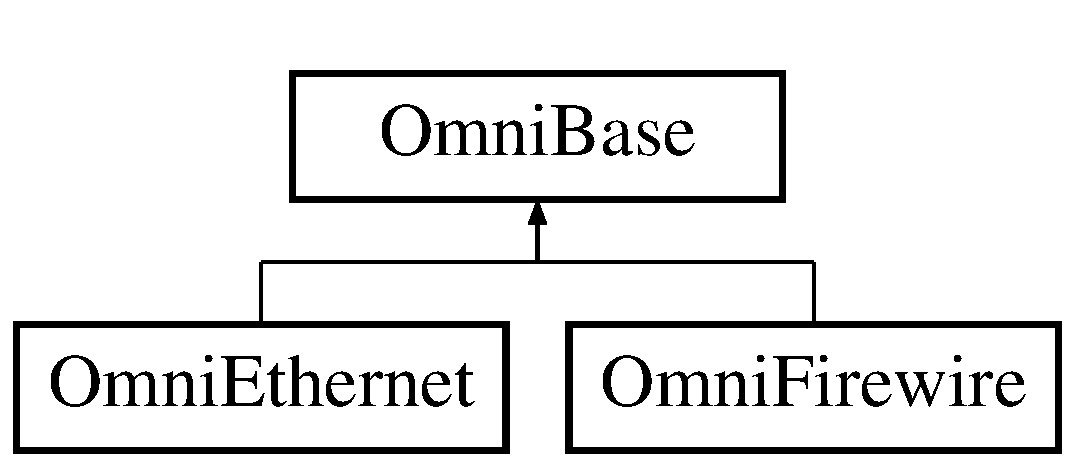
\includegraphics[height=2.000000cm]{classOmniBase}
\end{center}
\end{figure}
\subsection*{Classes}
\begin{DoxyCompactItemize}
\item 
struct \hyperlink{structOmniBase_1_1OmniState}{Omni\-State}
\begin{DoxyCompactList}\small\item\em $<$ The state structure with relevant data. \end{DoxyCompactList}\end{DoxyCompactItemize}
\subsection*{Public Member Functions}
\begin{DoxyCompactItemize}
\item 
\hyperlink{classOmniBase_ab8717851c5496b3311ba0b48114e8004}{Omni\-Base} (const std\-::string \&\hyperlink{classOmniBase_a69efd9c11cdef64cbdcf57b52c6539f7}{name}=\char`\"{}\char`\"{})
\begin{DoxyCompactList}\small\item\em \hyperlink{classOmniBase}{Omni\-Base} constructor, sets some members and prepares ros topics and publishers. \end{DoxyCompactList}\item 
\hypertarget{classOmniBase_afd21d9d7906e46cb6feb4d963bf8b9c7}{void \hyperlink{classOmniBase_afd21d9d7906e46cb6feb4d963bf8b9c7}{publish\-Omni\-State} ()}\label{classOmniBase_afd21d9d7906e46cb6feb4d963bf8b9c7}

\begin{DoxyCompactList}\small\item\em Publishes the current robot's state. \end{DoxyCompactList}\item 
virtual bool \hyperlink{classOmniBase_a60f376af41716a697ea79753160c3ca7}{connect} ()=0
\begin{DoxyCompactList}\small\item\em Attempts to connect to the robot. \end{DoxyCompactList}\item 
virtual void \hyperlink{classOmniBase_a7ba2a80063858d1cf7d5b03f9796ced4}{disconnect} ()=0
\begin{DoxyCompactList}\small\item\em Attempts to close the connection to the robot. \end{DoxyCompactList}\item 
virtual bool \hyperlink{classOmniBase_a22df750b9563aa7956950698e7463660}{connected} ()=0
\begin{DoxyCompactList}\small\item\em Checks if the device is connected. \end{DoxyCompactList}\item 
void \hyperlink{classOmniBase_aad2a1a9f26e79fd83b66aa8a0687b2fe}{get\-Joint\-Angles} (std\-::vector$<$ double $>$ \&angles)
\begin{DoxyCompactList}\small\item\em Gets the current joint angles. \end{DoxyCompactList}\item 
void \hyperlink{classOmniBase_a81bc07c9e555ffd56c2e9875fb02a5f3}{get\-Buttons\-State} (std\-::vector$<$ bool $>$ \&button)
\begin{DoxyCompactList}\small\item\em Gets the current buttons' state. \end{DoxyCompactList}\item 
void \hyperlink{classOmniBase_a2063df1014b3929d67c651fd72254d9f}{get\-Force} (std\-::vector$<$ double $>$ \&force)
\begin{DoxyCompactList}\small\item\em Gets the current force acting on the tip. \end{DoxyCompactList}\item 
void \hyperlink{classOmniBase_a6cae32aaf35f41719956c1f4e58f15e0}{set\-Torque} (const std\-::vector$<$ double $>$ \&torque)
\begin{DoxyCompactList}\small\item\em Sets the torque on the first three joints. \end{DoxyCompactList}\item 
void \hyperlink{classOmniBase_af5bd87d6589d31d88080f51f23b589df}{reset\-Torque} ()
\begin{DoxyCompactList}\small\item\em Resets the torque on the first three joints. \end{DoxyCompactList}\item 
void \hyperlink{classOmniBase_a1665798fd79dd5fb09a86e054364d5ce}{enable\-Control} (bool enable)
\begin{DoxyCompactList}\small\item\em Chooses if the control on the first three joints is on. \end{DoxyCompactList}\item 
void \hyperlink{classOmniBase_a81b7e2a28ea342cd956b549c8478c4c2}{get\-Joint\-Velocities} (std\-::vector$<$ double $>$ \&vel)
\begin{DoxyCompactList}\small\item\em Gets the current joint velocities. \end{DoxyCompactList}\item 
void \hyperlink{classOmniBase_a633d60e797f463662e7e43fa26ab339a}{get\-Tip\-Position} (std\-::vector$<$ double $>$ \&pos)
\begin{DoxyCompactList}\small\item\em Gets the current tip position with respect to the robot's base frame. \end{DoxyCompactList}\item 
void \hyperlink{classOmniBase_ab5a4cfa7473ec7ec301d6fa8565693f1}{get\-Tip\-Orientation} (std\-::vector$<$ double $>$ \&ori)
\begin{DoxyCompactList}\small\item\em Gets the current tip orientation with respect to the robot's base frame. \end{DoxyCompactList}\item 
void \hyperlink{classOmniBase_a19382d9187bca9ad3be17b8b5f5578ef}{get\-Tip\-Pose} (std\-::vector$<$ double $>$ \&pos, std\-::vector$<$ double $>$ \&ori)
\begin{DoxyCompactList}\small\item\em Gets the current tip position and orientation with respect to the robot's base frame. \end{DoxyCompactList}\item 
std\-::string \hyperlink{classOmniBase_ac5e0bcd250af6cc9a7396fa9306519ec}{get\-Topic\-Name} ()
\begin{DoxyCompactList}\small\item\em Gets the omni name param. \end{DoxyCompactList}\item 
bool \hyperlink{classOmniBase_a1b7f1a5010a0676f3446aa6adab1aaa4}{calibrated} ()
\begin{DoxyCompactList}\small\item\em Checks if the device has been calibrated. \end{DoxyCompactList}\item 
void \hyperlink{classOmniBase_a3bec44a6c7adfe6343eb56f20171f08e}{torque\-Callback} (const geometry\-\_\-msgs\-::\-Vector3\-::\-Const\-Ptr \&msg)
\begin{DoxyCompactList}\small\item\em The torque\-Callback called by the R\-O\-S torque subscriber. \end{DoxyCompactList}\item 
void \hyperlink{classOmniBase_ada27c388676a85ab31650cd2c1f8c068}{enable\-Control\-Callback} (const std\-\_\-msgs\-::\-Bool\-::\-Const\-Ptr \&msg)
\begin{DoxyCompactList}\small\item\em The enable\-Control\-Callback called by the R\-O\-S enable control subscriber. \end{DoxyCompactList}\end{DoxyCompactItemize}
\subsection*{Protected Types}
\begin{DoxyCompactItemize}
\item 
\hypertarget{classOmniBase_a46bff542660db9dadc41f044159b3b6a}{typedef \\*
boost\-::posix\-\_\-time\-::microsec\-\_\-clock {\bfseries Clock}}\label{classOmniBase_a46bff542660db9dadc41f044159b3b6a}

\item 
\hypertarget{classOmniBase_a4e45d98f32711195ffee4cfaadb535e9}{typedef boost\-::posix\-\_\-time\-::ptime {\bfseries Time}}\label{classOmniBase_a4e45d98f32711195ffee4cfaadb535e9}

\item 
\hypertarget{classOmniBase_accb4adedacf66489514f1a9fd9d564a4}{typedef \\*
boost\-::posix\-\_\-time\-::time\-\_\-duration {\bfseries Time\-Duration}}\label{classOmniBase_accb4adedacf66489514f1a9fd9d564a4}

\item 
\hypertarget{classOmniBase_ad03370b447b9b46cb62d6ebb002d7c37}{typedef boost\-::unique\-\_\-lock\\*
$<$ boost\-::shared\-\_\-mutex $>$ \hyperlink{classOmniBase_ad03370b447b9b46cb62d6ebb002d7c37}{Lock\-Unique}}\label{classOmniBase_ad03370b447b9b46cb62d6ebb002d7c37}

\begin{DoxyCompactList}\small\item\em The unique lock, used to protect data while writing. \end{DoxyCompactList}\item 
\hypertarget{classOmniBase_af9820aff8dc6ff7e8120bde218d557ca}{typedef boost\-::shared\-\_\-lock\\*
$<$ boost\-::shared\-\_\-mutex $>$ \hyperlink{classOmniBase_af9820aff8dc6ff7e8120bde218d557ca}{Lock\-Shared}}\label{classOmniBase_af9820aff8dc6ff7e8120bde218d557ca}

\begin{DoxyCompactList}\small\item\em The shared lock, used to protect data while reading. \end{DoxyCompactList}\item 
\hypertarget{classOmniBase_a7c9de7ece34c2c51e6922925fe5f11d7}{typedef boost\-::upgrade\-\_\-lock\\*
$<$ boost\-::shared\-\_\-mutex $>$ \hyperlink{classOmniBase_a7c9de7ece34c2c51e6922925fe5f11d7}{Lock\-Upgrade}}\label{classOmniBase_a7c9de7ece34c2c51e6922925fe5f11d7}

\begin{DoxyCompactList}\small\item\em The upgradeable lock, used to protect data while reading. \end{DoxyCompactList}\item 
\hypertarget{classOmniBase_a017d027fa1c72afe7b13c91869325364}{typedef \\*
boost\-::upgrade\-\_\-to\-\_\-unique\-\_\-lock\\*
$<$ boost\-::shared\-\_\-mutex $>$ \hyperlink{classOmniBase_a017d027fa1c72afe7b13c91869325364}{Lock\-Upgrade\-To\-Unique}}\label{classOmniBase_a017d027fa1c72afe7b13c91869325364}

\begin{DoxyCompactList}\small\item\em The upgraded lock, used to protect data while writing. \end{DoxyCompactList}\end{DoxyCompactItemize}
\subsection*{Protected Member Functions}
\begin{DoxyCompactItemize}
\item 
boost\-::shared\-\_\-mutex \& \hyperlink{classOmniBase_ae742a01f62b6e312c4704eea0d250f9d}{get\-State\-Mutex} ()
\begin{DoxyCompactList}\small\item\em Gets the mutex used for accessing the robot's state. \end{DoxyCompactList}\item 
\hyperlink{structOmniBase_1_1OmniState}{Omni\-State} $\ast$ \hyperlink{classOmniBase_a5c0ece986d3fbfa05331d0c885051134}{get\-State} ()
\begin{DoxyCompactList}\small\item\em Gets the robot's state. \end{DoxyCompactList}\end{DoxyCompactItemize}
\subsection*{Protected Attributes}
\begin{DoxyCompactItemize}
\item 
\hypertarget{classOmniBase_acfbd44decc32ec4af3eeca3e25281e45}{\hyperlink{structOmniBase_1_1OmniState}{Omni\-State} {\bfseries state}}\label{classOmniBase_acfbd44decc32ec4af3eeca3e25281e45}

\item 
\hypertarget{classOmniBase_a69efd9c11cdef64cbdcf57b52c6539f7}{std\-::string \hyperlink{classOmniBase_a69efd9c11cdef64cbdcf57b52c6539f7}{name}}\label{classOmniBase_a69efd9c11cdef64cbdcf57b52c6539f7}

\begin{DoxyCompactList}\small\item\em Name given to diferentiate multiple omnis. \end{DoxyCompactList}\item 
\hypertarget{classOmniBase_aad7cbf8f7beffd367ab50c3453e8d459}{std\-::string \hyperlink{classOmniBase_aad7cbf8f7beffd367ab50c3453e8d459}{topic\-\_\-name}}\label{classOmniBase_aad7cbf8f7beffd367ab50c3453e8d459}

\begin{DoxyCompactList}\small\item\em String used to subscribe diferent topics. \end{DoxyCompactList}\item 
\hypertarget{classOmniBase_a6bd8b4515724498791325d07caa849de}{ros\-::\-Node\-Handle\-Ptr {\bfseries node}}\label{classOmniBase_a6bd8b4515724498791325d07caa849de}

\item 
\hypertarget{classOmniBase_aca7da5f50524b6ad3d08deb11be59e2d}{ros\-::\-Subscriber \hyperlink{classOmniBase_aca7da5f50524b6ad3d08deb11be59e2d}{sub\-\_\-torque}}\label{classOmniBase_aca7da5f50524b6ad3d08deb11be59e2d}

\begin{DoxyCompactList}\small\item\em Torque R\-O\-S subscriber. \end{DoxyCompactList}\item 
\hypertarget{classOmniBase_a19970fdd4e693296f33fea90e8080033}{ros\-::\-Subscriber \hyperlink{classOmniBase_a19970fdd4e693296f33fea90e8080033}{sub\-\_\-enable\-\_\-control}}\label{classOmniBase_a19970fdd4e693296f33fea90e8080033}

\begin{DoxyCompactList}\small\item\em Enable control R\-O\-S subscriber. \end{DoxyCompactList}\item 
\hypertarget{classOmniBase_a60598eb25c3e6a1167fcbbdae581f1a5}{ros\-::\-Subscriber \hyperlink{classOmniBase_a60598eb25c3e6a1167fcbbdae581f1a5}{sub\-\_\-haptic}}\label{classOmniBase_a60598eb25c3e6a1167fcbbdae581f1a5}

\begin{DoxyCompactList}\small\item\em Enable haptic R\-O\-S subscriber. \end{DoxyCompactList}\item 
\hypertarget{classOmniBase_a610f935950307a0395c07d36313809b7}{ros\-::\-Publisher \hyperlink{classOmniBase_a610f935950307a0395c07d36313809b7}{pub\-\_\-joint}}\label{classOmniBase_a610f935950307a0395c07d36313809b7}

\begin{DoxyCompactList}\small\item\em Joint R\-O\-S publisher. \end{DoxyCompactList}\item 
\hypertarget{classOmniBase_ac4302b7badb135c465b71cb2d67b1a85}{sensor\-\_\-msgs\-::\-Joint\-State {\bfseries joint\-\_\-state}}\label{classOmniBase_ac4302b7badb135c465b71cb2d67b1a85}

\item 
\hypertarget{classOmniBase_ad8d0103682a01ed2a635f6aa01fb0124}{ros\-::\-Publisher \hyperlink{classOmniBase_ad8d0103682a01ed2a635f6aa01fb0124}{pub\-\_\-pose}}\label{classOmniBase_ad8d0103682a01ed2a635f6aa01fb0124}

\begin{DoxyCompactList}\small\item\em Pose R\-O\-S publisher. \end{DoxyCompactList}\item 
\hypertarget{classOmniBase_a0e3d2a98eb5be64e37dcce8939b99fe8}{geometry\-\_\-msgs\-::\-Pose\-Stamped {\bfseries pose\-\_\-stamped}}\label{classOmniBase_a0e3d2a98eb5be64e37dcce8939b99fe8}

\item 
\hypertarget{classOmniBase_a1cbe27fd9e63d07a9875e82a581bfab5}{ros\-::\-Publisher \hyperlink{classOmniBase_a1cbe27fd9e63d07a9875e82a581bfab5}{pub\-\_\-button}}\label{classOmniBase_a1cbe27fd9e63d07a9875e82a581bfab5}

\begin{DoxyCompactList}\small\item\em Button R\-O\-S publisher. \end{DoxyCompactList}\item 
\hypertarget{classOmniBase_aad994dc88b576231e3f37c11f510b319}{omni\-\_\-driver\-::\-Omni\-Button\-Event {\bfseries button\-\_\-event}}\label{classOmniBase_aad994dc88b576231e3f37c11f510b319}

\item 
\hypertarget{classOmniBase_acfbeb777f0f48bd79e18a57fa0d78d29}{bool \hyperlink{classOmniBase_acfbeb777f0f48bd79e18a57fa0d78d29}{last\-\_\-buttons} \mbox{[}2\mbox{]}}\label{classOmniBase_acfbeb777f0f48bd79e18a57fa0d78d29}

\begin{DoxyCompactList}\small\item\em Needed for \char`\"{}\-Button Clicked\char`\"{} logic. \end{DoxyCompactList}\item 
\hypertarget{classOmniBase_a2f35fcfb594e7be1bf22fcc3c3330348}{bool \hyperlink{classOmniBase_a2f35fcfb594e7be1bf22fcc3c3330348}{enable\-\_\-force\-\_\-flag}}\label{classOmniBase_a2f35fcfb594e7be1bf22fcc3c3330348}

\begin{DoxyCompactList}\small\item\em Needed for resetting the internal enable control. \end{DoxyCompactList}\end{DoxyCompactItemize}


\subsection{Constructor \& Destructor Documentation}
\hypertarget{classOmniBase_ab8717851c5496b3311ba0b48114e8004}{\index{Omni\-Base@{Omni\-Base}!Omni\-Base@{Omni\-Base}}
\index{Omni\-Base@{Omni\-Base}!OmniBase@{Omni\-Base}}
\subsubsection[{Omni\-Base}]{\setlength{\rightskip}{0pt plus 5cm}Omni\-Base\-::\-Omni\-Base (
\begin{DoxyParamCaption}
\item[{const std\-::string \&}]{name = {\ttfamily \char`\"{}\char`\"{}}}
\end{DoxyParamCaption}
)\hspace{0.3cm}{\ttfamily [explicit]}}}\label{classOmniBase_ab8717851c5496b3311ba0b48114e8004}


\hyperlink{classOmniBase}{Omni\-Base} constructor, sets some members and prepares ros topics and publishers. 


\begin{DoxyParams}{Parameters}
{\em name} & Reference to string of omni name. \\
\hline
\end{DoxyParams}


\subsection{Member Function Documentation}
\hypertarget{classOmniBase_a1b7f1a5010a0676f3446aa6adab1aaa4}{\index{Omni\-Base@{Omni\-Base}!calibrated@{calibrated}}
\index{calibrated@{calibrated}!OmniBase@{Omni\-Base}}
\subsubsection[{calibrated}]{\setlength{\rightskip}{0pt plus 5cm}bool Omni\-Base\-::calibrated (
\begin{DoxyParamCaption}
{}
\end{DoxyParamCaption}
)\hspace{0.3cm}{\ttfamily [inline]}}}\label{classOmniBase_a1b7f1a5010a0676f3446aa6adab1aaa4}


Checks if the device has been calibrated. 

\begin{DoxyReturn}{Returns}
True if calibrated. False otherwise. 
\end{DoxyReturn}
\hypertarget{classOmniBase_a60f376af41716a697ea79753160c3ca7}{\index{Omni\-Base@{Omni\-Base}!connect@{connect}}
\index{connect@{connect}!OmniBase@{Omni\-Base}}
\subsubsection[{connect}]{\setlength{\rightskip}{0pt plus 5cm}virtual bool Omni\-Base\-::connect (
\begin{DoxyParamCaption}
{}
\end{DoxyParamCaption}
)\hspace{0.3cm}{\ttfamily [pure virtual]}}}\label{classOmniBase_a60f376af41716a697ea79753160c3ca7}


Attempts to connect to the robot. 

\begin{DoxyReturn}{Returns}
True if the connection succeeds. False otherwise. 
\end{DoxyReturn}


Implemented in \hyperlink{classOmniFirewire_a5159a261f8a2a8a1e23e21ffc8b7d6d7}{Omni\-Firewire}, and \hyperlink{classOmniEthernet_a2c066f15ef8554fb34ad7901101fa623}{Omni\-Ethernet}.

\hypertarget{classOmniBase_a22df750b9563aa7956950698e7463660}{\index{Omni\-Base@{Omni\-Base}!connected@{connected}}
\index{connected@{connected}!OmniBase@{Omni\-Base}}
\subsubsection[{connected}]{\setlength{\rightskip}{0pt plus 5cm}virtual bool Omni\-Base\-::connected (
\begin{DoxyParamCaption}
{}
\end{DoxyParamCaption}
)\hspace{0.3cm}{\ttfamily [pure virtual]}}}\label{classOmniBase_a22df750b9563aa7956950698e7463660}


Checks if the device is connected. 

\begin{DoxyReturn}{Returns}
True if connected. False otherwise. 
\end{DoxyReturn}
\begin{DoxySeeAlso}{See Also}
\hyperlink{classOmniBase_a60f376af41716a697ea79753160c3ca7}{connect}, \hyperlink{classOmniBase_a7ba2a80063858d1cf7d5b03f9796ced4}{disconnect} 
\end{DoxySeeAlso}


Implemented in \hyperlink{classOmniEthernet_aee413137593a3231deeb304537d80d05}{Omni\-Ethernet}.

\hypertarget{classOmniBase_a7ba2a80063858d1cf7d5b03f9796ced4}{\index{Omni\-Base@{Omni\-Base}!disconnect@{disconnect}}
\index{disconnect@{disconnect}!OmniBase@{Omni\-Base}}
\subsubsection[{disconnect}]{\setlength{\rightskip}{0pt plus 5cm}virtual void Omni\-Base\-::disconnect (
\begin{DoxyParamCaption}
{}
\end{DoxyParamCaption}
)\hspace{0.3cm}{\ttfamily [pure virtual]}}}\label{classOmniBase_a7ba2a80063858d1cf7d5b03f9796ced4}


Attempts to close the connection to the robot. 

\begin{DoxyReturn}{Returns}
True if the connection was closed. False otherwise. 
\end{DoxyReturn}


Implemented in \hyperlink{classOmniFirewire_a7e8c7caaa494c1e0024cc3dbdeab5eee}{Omni\-Firewire}, and \hyperlink{classOmniEthernet_aba4911f37396e1b1f09f7e5b28ea105f}{Omni\-Ethernet}.

\hypertarget{classOmniBase_a1665798fd79dd5fb09a86e054364d5ce}{\index{Omni\-Base@{Omni\-Base}!enable\-Control@{enable\-Control}}
\index{enable\-Control@{enable\-Control}!OmniBase@{Omni\-Base}}
\subsubsection[{enable\-Control}]{\setlength{\rightskip}{0pt plus 5cm}void Omni\-Base\-::enable\-Control (
\begin{DoxyParamCaption}
\item[{bool}]{enable}
\end{DoxyParamCaption}
)\hspace{0.3cm}{\ttfamily [inline]}}}\label{classOmniBase_a1665798fd79dd5fb09a86e054364d5ce}


Chooses if the control on the first three joints is on. 


\begin{DoxyParams}{Parameters}
{\em enable} & True to enable. False otherwise. \\
\hline
\end{DoxyParams}
\hypertarget{classOmniBase_ada27c388676a85ab31650cd2c1f8c068}{\index{Omni\-Base@{Omni\-Base}!enable\-Control\-Callback@{enable\-Control\-Callback}}
\index{enable\-Control\-Callback@{enable\-Control\-Callback}!OmniBase@{Omni\-Base}}
\subsubsection[{enable\-Control\-Callback}]{\setlength{\rightskip}{0pt plus 5cm}void Omni\-Base\-::enable\-Control\-Callback (
\begin{DoxyParamCaption}
\item[{const std\-\_\-msgs\-::\-Bool\-::\-Const\-Ptr \&}]{msg}
\end{DoxyParamCaption}
)}}\label{classOmniBase_ada27c388676a85ab31650cd2c1f8c068}


The enable\-Control\-Callback called by the R\-O\-S enable control subscriber. 


\begin{DoxyParams}{Parameters}
{\em R\-O\-S} & message type geometry\-\_\-msgs\-::\-Bool. \\
\hline
\end{DoxyParams}
\hypertarget{classOmniBase_a81bc07c9e555ffd56c2e9875fb02a5f3}{\index{Omni\-Base@{Omni\-Base}!get\-Buttons\-State@{get\-Buttons\-State}}
\index{get\-Buttons\-State@{get\-Buttons\-State}!OmniBase@{Omni\-Base}}
\subsubsection[{get\-Buttons\-State}]{\setlength{\rightskip}{0pt plus 5cm}void Omni\-Base\-::get\-Buttons\-State (
\begin{DoxyParamCaption}
\item[{std\-::vector$<$ bool $>$ \&}]{button}
\end{DoxyParamCaption}
)\hspace{0.3cm}{\ttfamily [inline]}}}\label{classOmniBase_a81bc07c9e555ffd56c2e9875fb02a5f3}


Gets the current buttons' state. 


\begin{DoxyParams}{Parameters}
{\em button} & Vector that will store the states. \\
\hline
\end{DoxyParams}
\hypertarget{classOmniBase_a2063df1014b3929d67c651fd72254d9f}{\index{Omni\-Base@{Omni\-Base}!get\-Force@{get\-Force}}
\index{get\-Force@{get\-Force}!OmniBase@{Omni\-Base}}
\subsubsection[{get\-Force}]{\setlength{\rightskip}{0pt plus 5cm}void Omni\-Base\-::get\-Force (
\begin{DoxyParamCaption}
\item[{std\-::vector$<$ double $>$ \&}]{force}
\end{DoxyParamCaption}
)\hspace{0.3cm}{\ttfamily [inline]}}}\label{classOmniBase_a2063df1014b3929d67c651fd72254d9f}


Gets the current force acting on the tip. 


\begin{DoxyParams}{Parameters}
{\em force} & Vector that will store the force. \\
\hline
\end{DoxyParams}
\hypertarget{classOmniBase_aad2a1a9f26e79fd83b66aa8a0687b2fe}{\index{Omni\-Base@{Omni\-Base}!get\-Joint\-Angles@{get\-Joint\-Angles}}
\index{get\-Joint\-Angles@{get\-Joint\-Angles}!OmniBase@{Omni\-Base}}
\subsubsection[{get\-Joint\-Angles}]{\setlength{\rightskip}{0pt plus 5cm}void Omni\-Base\-::get\-Joint\-Angles (
\begin{DoxyParamCaption}
\item[{std\-::vector$<$ double $>$ \&}]{angles}
\end{DoxyParamCaption}
)\hspace{0.3cm}{\ttfamily [inline]}}}\label{classOmniBase_aad2a1a9f26e79fd83b66aa8a0687b2fe}


Gets the current joint angles. 


\begin{DoxyParams}{Parameters}
{\em angles} & Vector that will store the angles. \\
\hline
\end{DoxyParams}
\hypertarget{classOmniBase_a81b7e2a28ea342cd956b549c8478c4c2}{\index{Omni\-Base@{Omni\-Base}!get\-Joint\-Velocities@{get\-Joint\-Velocities}}
\index{get\-Joint\-Velocities@{get\-Joint\-Velocities}!OmniBase@{Omni\-Base}}
\subsubsection[{get\-Joint\-Velocities}]{\setlength{\rightskip}{0pt plus 5cm}void Omni\-Base\-::get\-Joint\-Velocities (
\begin{DoxyParamCaption}
\item[{std\-::vector$<$ double $>$ \&}]{vel}
\end{DoxyParamCaption}
)\hspace{0.3cm}{\ttfamily [inline]}}}\label{classOmniBase_a81b7e2a28ea342cd956b549c8478c4c2}


Gets the current joint velocities. 


\begin{DoxyParams}{Parameters}
{\em vel} & Vector that will store the velocities. \\
\hline
\end{DoxyParams}
\hypertarget{classOmniBase_a5c0ece986d3fbfa05331d0c885051134}{\index{Omni\-Base@{Omni\-Base}!get\-State@{get\-State}}
\index{get\-State@{get\-State}!OmniBase@{Omni\-Base}}
\subsubsection[{get\-State}]{\setlength{\rightskip}{0pt plus 5cm}{\bf Omni\-State}$\ast$ Omni\-Base\-::get\-State (
\begin{DoxyParamCaption}
{}
\end{DoxyParamCaption}
)\hspace{0.3cm}{\ttfamily [inline]}, {\ttfamily [protected]}}}\label{classOmniBase_a5c0ece986d3fbfa05331d0c885051134}


Gets the robot's state. 

\begin{DoxyReturn}{Returns}
The robot's state. 
\end{DoxyReturn}
\hypertarget{classOmniBase_ae742a01f62b6e312c4704eea0d250f9d}{\index{Omni\-Base@{Omni\-Base}!get\-State\-Mutex@{get\-State\-Mutex}}
\index{get\-State\-Mutex@{get\-State\-Mutex}!OmniBase@{Omni\-Base}}
\subsubsection[{get\-State\-Mutex}]{\setlength{\rightskip}{0pt plus 5cm}boost\-::shared\-\_\-mutex\& Omni\-Base\-::get\-State\-Mutex (
\begin{DoxyParamCaption}
{}
\end{DoxyParamCaption}
)\hspace{0.3cm}{\ttfamily [inline]}, {\ttfamily [protected]}}}\label{classOmniBase_ae742a01f62b6e312c4704eea0d250f9d}


Gets the mutex used for accessing the robot's state. 

\begin{DoxyReturn}{Returns}
The mutex. 
\end{DoxyReturn}
\hypertarget{classOmniBase_ab5a4cfa7473ec7ec301d6fa8565693f1}{\index{Omni\-Base@{Omni\-Base}!get\-Tip\-Orientation@{get\-Tip\-Orientation}}
\index{get\-Tip\-Orientation@{get\-Tip\-Orientation}!OmniBase@{Omni\-Base}}
\subsubsection[{get\-Tip\-Orientation}]{\setlength{\rightskip}{0pt plus 5cm}void Omni\-Base\-::get\-Tip\-Orientation (
\begin{DoxyParamCaption}
\item[{std\-::vector$<$ double $>$ \&}]{ori}
\end{DoxyParamCaption}
)\hspace{0.3cm}{\ttfamily [inline]}}}\label{classOmniBase_ab5a4cfa7473ec7ec301d6fa8565693f1}


Gets the current tip orientation with respect to the robot's base frame. 


\begin{DoxyParams}{Parameters}
{\em ori} & Vector that will store the orientation as a quaternion. \\
\hline
\end{DoxyParams}
\hypertarget{classOmniBase_a19382d9187bca9ad3be17b8b5f5578ef}{\index{Omni\-Base@{Omni\-Base}!get\-Tip\-Pose@{get\-Tip\-Pose}}
\index{get\-Tip\-Pose@{get\-Tip\-Pose}!OmniBase@{Omni\-Base}}
\subsubsection[{get\-Tip\-Pose}]{\setlength{\rightskip}{0pt plus 5cm}void Omni\-Base\-::get\-Tip\-Pose (
\begin{DoxyParamCaption}
\item[{std\-::vector$<$ double $>$ \&}]{pos, }
\item[{std\-::vector$<$ double $>$ \&}]{ori}
\end{DoxyParamCaption}
)\hspace{0.3cm}{\ttfamily [inline]}}}\label{classOmniBase_a19382d9187bca9ad3be17b8b5f5578ef}


Gets the current tip position and orientation with respect to the robot's base frame. 


\begin{DoxyParams}{Parameters}
{\em pos} & Vector that will store the position. \\
\hline
{\em ori} & Vector that will store the orientation as a quaternion. \\
\hline
\end{DoxyParams}
\begin{DoxySeeAlso}{See Also}
\hyperlink{classOmniBase_a633d60e797f463662e7e43fa26ab339a}{get\-Tip\-Position}, \hyperlink{classOmniBase_ab5a4cfa7473ec7ec301d6fa8565693f1}{get\-Tip\-Orientation} 
\end{DoxySeeAlso}
\hypertarget{classOmniBase_a633d60e797f463662e7e43fa26ab339a}{\index{Omni\-Base@{Omni\-Base}!get\-Tip\-Position@{get\-Tip\-Position}}
\index{get\-Tip\-Position@{get\-Tip\-Position}!OmniBase@{Omni\-Base}}
\subsubsection[{get\-Tip\-Position}]{\setlength{\rightskip}{0pt plus 5cm}void Omni\-Base\-::get\-Tip\-Position (
\begin{DoxyParamCaption}
\item[{std\-::vector$<$ double $>$ \&}]{pos}
\end{DoxyParamCaption}
)\hspace{0.3cm}{\ttfamily [inline]}}}\label{classOmniBase_a633d60e797f463662e7e43fa26ab339a}


Gets the current tip position with respect to the robot's base frame. 


\begin{DoxyParams}{Parameters}
{\em pos} & Vector that will store the position. \\
\hline
\end{DoxyParams}
\hypertarget{classOmniBase_ac5e0bcd250af6cc9a7396fa9306519ec}{\index{Omni\-Base@{Omni\-Base}!get\-Topic\-Name@{get\-Topic\-Name}}
\index{get\-Topic\-Name@{get\-Topic\-Name}!OmniBase@{Omni\-Base}}
\subsubsection[{get\-Topic\-Name}]{\setlength{\rightskip}{0pt plus 5cm}std\-::string Omni\-Base\-::get\-Topic\-Name (
\begin{DoxyParamCaption}
{}
\end{DoxyParamCaption}
)\hspace{0.3cm}{\ttfamily [inline]}}}\label{classOmniBase_ac5e0bcd250af6cc9a7396fa9306519ec}


Gets the omni name param. 

\begin{DoxyReturn}{Returns}
Returns the robot's name. 
\end{DoxyReturn}
\hypertarget{classOmniBase_af5bd87d6589d31d88080f51f23b589df}{\index{Omni\-Base@{Omni\-Base}!reset\-Torque@{reset\-Torque}}
\index{reset\-Torque@{reset\-Torque}!OmniBase@{Omni\-Base}}
\subsubsection[{reset\-Torque}]{\setlength{\rightskip}{0pt plus 5cm}void Omni\-Base\-::reset\-Torque (
\begin{DoxyParamCaption}
{}
\end{DoxyParamCaption}
)\hspace{0.3cm}{\ttfamily [inline]}}}\label{classOmniBase_af5bd87d6589d31d88080f51f23b589df}


Resets the torque on the first three joints. 

\begin{DoxySeeAlso}{See Also}
\hyperlink{classOmniBase_a6cae32aaf35f41719956c1f4e58f15e0}{set\-Torque} 
\end{DoxySeeAlso}
\hypertarget{classOmniBase_a6cae32aaf35f41719956c1f4e58f15e0}{\index{Omni\-Base@{Omni\-Base}!set\-Torque@{set\-Torque}}
\index{set\-Torque@{set\-Torque}!OmniBase@{Omni\-Base}}
\subsubsection[{set\-Torque}]{\setlength{\rightskip}{0pt plus 5cm}void Omni\-Base\-::set\-Torque (
\begin{DoxyParamCaption}
\item[{const std\-::vector$<$ double $>$ \&}]{torque}
\end{DoxyParamCaption}
)\hspace{0.3cm}{\ttfamily [inline]}}}\label{classOmniBase_a6cae32aaf35f41719956c1f4e58f15e0}


Sets the torque on the first three joints. 


\begin{DoxyParams}{Parameters}
{\em torque} & 3-\/elements vector with the torque values. \\
\hline
\end{DoxyParams}
\hypertarget{classOmniBase_a3bec44a6c7adfe6343eb56f20171f08e}{\index{Omni\-Base@{Omni\-Base}!torque\-Callback@{torque\-Callback}}
\index{torque\-Callback@{torque\-Callback}!OmniBase@{Omni\-Base}}
\subsubsection[{torque\-Callback}]{\setlength{\rightskip}{0pt plus 5cm}void Omni\-Base\-::torque\-Callback (
\begin{DoxyParamCaption}
\item[{const geometry\-\_\-msgs\-::\-Vector3\-::\-Const\-Ptr \&}]{msg}
\end{DoxyParamCaption}
)}}\label{classOmniBase_a3bec44a6c7adfe6343eb56f20171f08e}


The torque\-Callback called by the R\-O\-S torque subscriber. 


\begin{DoxyParams}{Parameters}
{\em R\-O\-S} & message type geometry\-\_\-msgs\-::\-Vector3. \\
\hline
\end{DoxyParams}


The documentation for this class was generated from the following files\-:\begin{DoxyCompactItemize}
\item 
include/omnibase.\-h\item 
src/omnibase.\-cpp\end{DoxyCompactItemize}

\hypertarget{classOmniEthernet}{\section{Omni\-Ethernet Class Reference}
\label{classOmniEthernet}\index{Omni\-Ethernet@{Omni\-Ethernet}}
}
Inheritance diagram for Omni\-Ethernet\-:\begin{figure}[H]
\begin{center}
\leavevmode
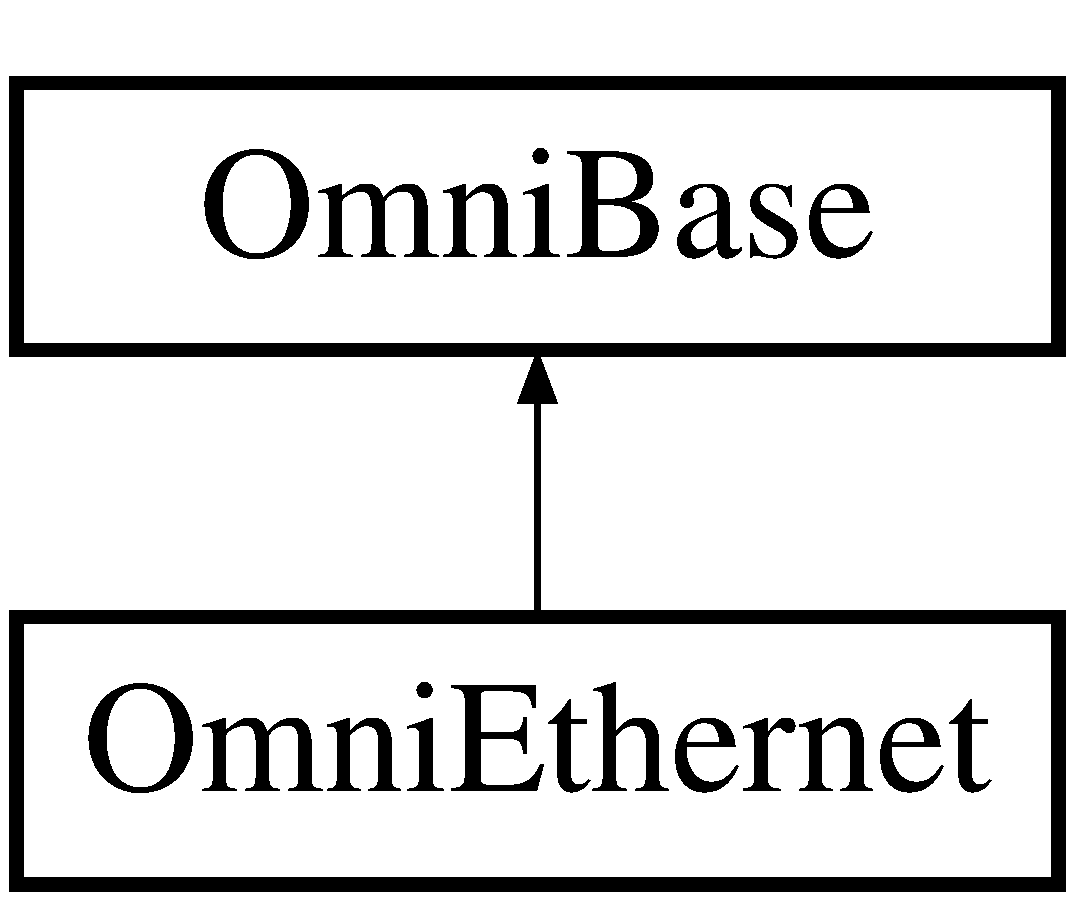
\includegraphics[height=2.000000cm]{classOmniEthernet}
\end{center}
\end{figure}
\subsection*{Public Member Functions}
\begin{DoxyCompactItemize}
\item 
bool \hyperlink{classOmniEthernet_a2c066f15ef8554fb34ad7901101fa623}{connect} ()
\begin{DoxyCompactList}\small\item\em Connects and calibrates to the device, starting the communication. \end{DoxyCompactList}\item 
bool \hyperlink{classOmniEthernet_aee413137593a3231deeb304537d80d05}{connected} ()
\begin{DoxyCompactList}\small\item\em Used to check if a device is connected. \end{DoxyCompactList}\item 
\hypertarget{classOmniEthernet_aba4911f37396e1b1f09f7e5b28ea105f}{void \hyperlink{classOmniEthernet_aba4911f37396e1b1f09f7e5b28ea105f}{disconnect} ()}\label{classOmniEthernet_aba4911f37396e1b1f09f7e5b28ea105f}

\begin{DoxyCompactList}\small\item\em Disconnects the device, called by destructor. \end{DoxyCompactList}\item 
\hyperlink{classOmniEthernet_a55e6473c599ca47a64d35f9194ad5603}{Omni\-Ethernet} (const std\-::string \&\hyperlink{classOmniBase_a69efd9c11cdef64cbdcf57b52c6539f7}{name}=\char`\"{}\char`\"{})
\begin{DoxyCompactList}\small\item\em \hyperlink{classOmniEthernet}{Omni\-Ethernet} constructor, calls \hyperlink{classOmniBase}{Omni\-Base} constructor with same parameter. \end{DoxyCompactList}\end{DoxyCompactItemize}
\subsection*{Static Public Attributes}
\begin{DoxyCompactItemize}
\item 
\hypertarget{classOmniEthernet_a1e1795bfe2ff731548c50bf6e7391f23}{static int {\bfseries calibration\-Style} = 0}\label{classOmniEthernet_a1e1795bfe2ff731548c50bf6e7391f23}

\end{DoxyCompactItemize}
\subsection*{Additional Inherited Members}


\subsection{Constructor \& Destructor Documentation}
\hypertarget{classOmniEthernet_a55e6473c599ca47a64d35f9194ad5603}{\index{Omni\-Ethernet@{Omni\-Ethernet}!Omni\-Ethernet@{Omni\-Ethernet}}
\index{Omni\-Ethernet@{Omni\-Ethernet}!OmniEthernet@{Omni\-Ethernet}}
\subsubsection[{Omni\-Ethernet}]{\setlength{\rightskip}{0pt plus 5cm}Omni\-Ethernet\-::\-Omni\-Ethernet (
\begin{DoxyParamCaption}
\item[{const std\-::string \&}]{name = {\ttfamily \char`\"{}\char`\"{}}}
\end{DoxyParamCaption}
)}}\label{classOmniEthernet_a55e6473c599ca47a64d35f9194ad5603}


\hyperlink{classOmniEthernet}{Omni\-Ethernet} constructor, calls \hyperlink{classOmniBase}{Omni\-Base} constructor with same parameter. 


\begin{DoxyParams}{Parameters}
{\em name} & Reference to string of omni name. \\
\hline
\end{DoxyParams}


\subsection{Member Function Documentation}
\hypertarget{classOmniEthernet_a2c066f15ef8554fb34ad7901101fa623}{\index{Omni\-Ethernet@{Omni\-Ethernet}!connect@{connect}}
\index{connect@{connect}!OmniEthernet@{Omni\-Ethernet}}
\subsubsection[{connect}]{\setlength{\rightskip}{0pt plus 5cm}bool Omni\-Ethernet\-::connect (
\begin{DoxyParamCaption}
{}
\end{DoxyParamCaption}
)\hspace{0.3cm}{\ttfamily [virtual]}}}\label{classOmniEthernet_a2c066f15ef8554fb34ad7901101fa623}


Connects and calibrates to the device, starting the communication. 

\begin{DoxyReturn}{Returns}
Return 1 if the connection was succesfull, 0 otherwise. 
\end{DoxyReturn}


Implements \hyperlink{classOmniBase_a60f376af41716a697ea79753160c3ca7}{Omni\-Base}.

\hypertarget{classOmniEthernet_aee413137593a3231deeb304537d80d05}{\index{Omni\-Ethernet@{Omni\-Ethernet}!connected@{connected}}
\index{connected@{connected}!OmniEthernet@{Omni\-Ethernet}}
\subsubsection[{connected}]{\setlength{\rightskip}{0pt plus 5cm}bool Omni\-Ethernet\-::connected (
\begin{DoxyParamCaption}
{}
\end{DoxyParamCaption}
)\hspace{0.3cm}{\ttfamily [virtual]}}}\label{classOmniEthernet_aee413137593a3231deeb304537d80d05}


Used to check if a device is connected. 

\begin{DoxyReturn}{Returns}
Returns 1 if a device connected, 0 otherwise. 
\end{DoxyReturn}


Implements \hyperlink{classOmniBase_a22df750b9563aa7956950698e7463660}{Omni\-Base}.



The documentation for this class was generated from the following files\-:\begin{DoxyCompactItemize}
\item 
include/omniethernet.\-h\item 
src/omniethernet.\-cpp\end{DoxyCompactItemize}

\hypertarget{classOmniFirewire}{\section{Omni\-Firewire Class Reference}
\label{classOmniFirewire}\index{Omni\-Firewire@{Omni\-Firewire}}
}
Inheritance diagram for Omni\-Firewire\-:\begin{figure}[H]
\begin{center}
\leavevmode
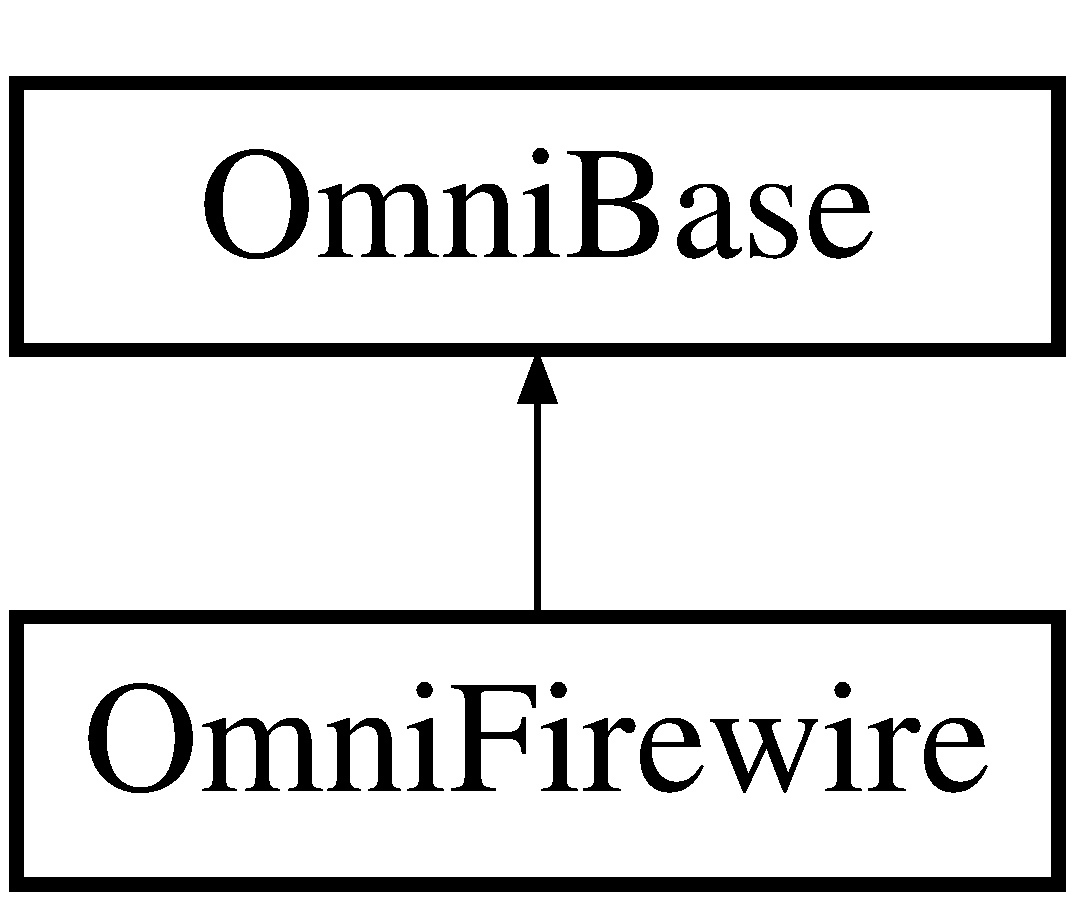
\includegraphics[height=2.000000cm]{classOmniFirewire}
\end{center}
\end{figure}
\subsection*{Classes}
\begin{DoxyCompactItemize}
\item 
struct \hyperlink{structOmniFirewire_1_1OmniInfo}{Omni\-Info}
\begin{DoxyCompactList}\small\item\em $<$ Structure with device connection information. \end{DoxyCompactList}\end{DoxyCompactItemize}
\subsection*{Public Member Functions}
\begin{DoxyCompactItemize}
\item 
bool \hyperlink{classOmniFirewire_a5159a261f8a2a8a1e23e21ffc8b7d6d7}{connect} ()
\begin{DoxyCompactList}\small\item\em Used to connect with omni device. \end{DoxyCompactList}\item 
\hypertarget{classOmniFirewire_a7e8c7caaa494c1e0024cc3dbdeab5eee}{void \hyperlink{classOmniFirewire_a7e8c7caaa494c1e0024cc3dbdeab5eee}{disconnect} ()}\label{classOmniFirewire_a7e8c7caaa494c1e0024cc3dbdeab5eee}

\begin{DoxyCompactList}\small\item\em Used to disconnect with omni device. \end{DoxyCompactList}\item 
\hyperlink{classOmniFirewire_af9298dc3107550d4da86e4eb12fdfe09}{Omni\-Firewire} (const std\-::string \&serial\-\_\-number, const std\-::string \&\hyperlink{classOmniBase_a69efd9c11cdef64cbdcf57b52c6539f7}{name}=\char`\"{}\char`\"{})
\begin{DoxyCompactList}\small\item\em \hyperlink{classOmniFirewire}{Omni\-Firewire} constructor, only sets some members needed for communicating with omni. \end{DoxyCompactList}\end{DoxyCompactItemize}
\subsection*{Static Public Member Functions}
\begin{DoxyCompactItemize}
\item 
static std\-::vector\\*
$<$ \hyperlink{structOmniFirewire_1_1OmniInfo}{Omni\-Firewire\-::\-Omni\-Info} $>$ \hyperlink{classOmniFirewire_a1862100a3027d7ea92342faa79751073}{enumerate\-\_\-omnis} ()
\begin{DoxyCompactList}\small\item\em Used to enumerate devices found. \end{DoxyCompactList}\end{DoxyCompactItemize}
\subsection*{Additional Inherited Members}


\subsection{Constructor \& Destructor Documentation}
\hypertarget{classOmniFirewire_af9298dc3107550d4da86e4eb12fdfe09}{\index{Omni\-Firewire@{Omni\-Firewire}!Omni\-Firewire@{Omni\-Firewire}}
\index{Omni\-Firewire@{Omni\-Firewire}!OmniFirewire@{Omni\-Firewire}}
\subsubsection[{Omni\-Firewire}]{\setlength{\rightskip}{0pt plus 5cm}Omni\-Firewire\-::\-Omni\-Firewire (
\begin{DoxyParamCaption}
\item[{const std\-::string \&}]{serial\-\_\-number, }
\item[{const std\-::string \&}]{name = {\ttfamily \char`\"{}\char`\"{}}}
\end{DoxyParamCaption}
)}}\label{classOmniFirewire_af9298dc3107550d4da86e4eb12fdfe09}


\hyperlink{classOmniFirewire}{Omni\-Firewire} constructor, only sets some members needed for communicating with omni. 


\begin{DoxyParams}{Parameters}
{\em serial\-\_\-number} & Reference to string of serial number. \\
\hline
{\em name} & Reference to string of omni name. \\
\hline
\end{DoxyParams}


\subsection{Member Function Documentation}
\hypertarget{classOmniFirewire_a5159a261f8a2a8a1e23e21ffc8b7d6d7}{\index{Omni\-Firewire@{Omni\-Firewire}!connect@{connect}}
\index{connect@{connect}!OmniFirewire@{Omni\-Firewire}}
\subsubsection[{connect}]{\setlength{\rightskip}{0pt plus 5cm}bool Omni\-Firewire\-::connect (
\begin{DoxyParamCaption}
{}
\end{DoxyParamCaption}
)\hspace{0.3cm}{\ttfamily [virtual]}}}\label{classOmniFirewire_a5159a261f8a2a8a1e23e21ffc8b7d6d7}


Used to connect with omni device. 

\begin{DoxyReturn}{Returns}
Returns 1 if successfull, 0 otherwise. 
\end{DoxyReturn}


Implements \hyperlink{classOmniBase_a60f376af41716a697ea79753160c3ca7}{Omni\-Base}.

\hypertarget{classOmniFirewire_a1862100a3027d7ea92342faa79751073}{\index{Omni\-Firewire@{Omni\-Firewire}!enumerate\-\_\-omnis@{enumerate\-\_\-omnis}}
\index{enumerate\-\_\-omnis@{enumerate\-\_\-omnis}!OmniFirewire@{Omni\-Firewire}}
\subsubsection[{enumerate\-\_\-omnis}]{\setlength{\rightskip}{0pt plus 5cm}std\-::vector$<$ {\bf Omni\-Firewire\-::\-Omni\-Info} $>$ Omni\-Firewire\-::enumerate\-\_\-omnis (
\begin{DoxyParamCaption}
{}
\end{DoxyParamCaption}
)\hspace{0.3cm}{\ttfamily [static]}}}\label{classOmniFirewire_a1862100a3027d7ea92342faa79751073}


Used to enumerate devices found. 

\begin{DoxyReturn}{Returns}
Returns a vector with information from different devices in the \hyperlink{structOmniFirewire_1_1OmniInfo}{Omni\-Info} struct format. 
\end{DoxyReturn}


The documentation for this class was generated from the following files\-:\begin{DoxyCompactItemize}
\item 
include/omnifirewire.\-h\item 
src/omnifirewire.\-cpp\end{DoxyCompactItemize}

\hypertarget{structOmniFirewire_1_1OmniInfo}{\section{Omni\-Firewire\-:\-:Omni\-Info Struct Reference}
\label{structOmniFirewire_1_1OmniInfo}\index{Omni\-Firewire\-::\-Omni\-Info@{Omni\-Firewire\-::\-Omni\-Info}}
}


$<$ Structure with device connection information.  




{\ttfamily \#include $<$omnifirewire.\-h$>$}

\subsection*{Public Member Functions}
\begin{DoxyCompactItemize}
\item 
\hypertarget{structOmniFirewire_1_1OmniInfo_a947a8907e1a1c6224f25238418faefaf}{{\bfseries Omni\-Info} (const std\-::string \&serial, int32\-\_\-t port, int32\-\_\-t node)}\label{structOmniFirewire_1_1OmniInfo_a947a8907e1a1c6224f25238418faefaf}

\end{DoxyCompactItemize}
\subsection*{Public Attributes}
\begin{DoxyCompactItemize}
\item 
\hypertarget{structOmniFirewire_1_1OmniInfo_a53552f6be728d8ef111252149dce7952}{std\-::string {\bfseries serial}}\label{structOmniFirewire_1_1OmniInfo_a53552f6be728d8ef111252149dce7952}

\item 
\hypertarget{structOmniFirewire_1_1OmniInfo_ac2e80f703a26bf811c7e0da1e723a4d5}{int32\-\_\-t {\bfseries port}}\label{structOmniFirewire_1_1OmniInfo_ac2e80f703a26bf811c7e0da1e723a4d5}

\item 
\hypertarget{structOmniFirewire_1_1OmniInfo_a3203599f79114093c8472fe297a961b1}{int32\-\_\-t {\bfseries node}}\label{structOmniFirewire_1_1OmniInfo_a3203599f79114093c8472fe297a961b1}

\end{DoxyCompactItemize}


\subsection{Detailed Description}
$<$ Structure with device connection information. 

The documentation for this struct was generated from the following file\-:\begin{DoxyCompactItemize}
\item 
include/omnifirewire.\-h\end{DoxyCompactItemize}

\hypertarget{structOmniBase_1_1OmniState}{\section{Omni\-Base\-:\-:Omni\-State Struct Reference}
\label{structOmniBase_1_1OmniState}\index{Omni\-Base\-::\-Omni\-State@{Omni\-Base\-::\-Omni\-State}}
}


$<$ The state structure with relevant data.  




{\ttfamily \#include $<$omnibase.\-h$>$}

\subsection*{Public Attributes}
\begin{DoxyCompactItemize}
\item 
\hypertarget{structOmniBase_1_1OmniState_a308df8149c1178f6614c6fa46b3a6f1e}{std\-::vector$<$ double $>$ {\bfseries angles}}\label{structOmniBase_1_1OmniState_a308df8149c1178f6614c6fa46b3a6f1e}

\item 
\hypertarget{structOmniBase_1_1OmniState_a8e21a0e1ec49c0200b0a643b6c925426}{std\-::vector$<$ double $>$ {\bfseries angles\-\_\-docked}}\label{structOmniBase_1_1OmniState_a8e21a0e1ec49c0200b0a643b6c925426}

\item 
\hypertarget{structOmniBase_1_1OmniState_a823efdd421f8ea426c6525200799b5e2}{std\-::vector$<$ double $>$ {\bfseries angles\-\_\-last}}\label{structOmniBase_1_1OmniState_a823efdd421f8ea426c6525200799b5e2}

\item 
\hypertarget{structOmniBase_1_1OmniState_a16f123e4a5da50cf94ec608a6f67c0d5}{std\-::vector$<$ double $>$ {\bfseries control}}\label{structOmniBase_1_1OmniState_a16f123e4a5da50cf94ec608a6f67c0d5}

\item 
\hypertarget{structOmniBase_1_1OmniState_a391320ee52a931aed7cb56e9b3bd5439}{std\-::vector$<$ double $>$ {\bfseries force}}\label{structOmniBase_1_1OmniState_a391320ee52a931aed7cb56e9b3bd5439}

\item 
\hypertarget{structOmniBase_1_1OmniState_a11ae38c471dd3e992677bfabb2168b1b}{std\-::vector$<$ double $>$ {\bfseries lock\-\_\-pos}}\label{structOmniBase_1_1OmniState_a11ae38c471dd3e992677bfabb2168b1b}

\item 
\hypertarget{structOmniBase_1_1OmniState_a83a16e0cd9d5c627733f710be60e0014}{std\-::vector$<$ double $>$ {\bfseries orientation}}\label{structOmniBase_1_1OmniState_a83a16e0cd9d5c627733f710be60e0014}

\item 
\hypertarget{structOmniBase_1_1OmniState_ac633ff71953171b841f5e23f53bfe162}{std\-::vector$<$ double $>$ {\bfseries position}}\label{structOmniBase_1_1OmniState_ac633ff71953171b841f5e23f53bfe162}

\item 
\hypertarget{structOmniBase_1_1OmniState_a9b9eeb34f926135c2c373a9a6c2b9081}{std\-::vector$<$ double $>$ {\bfseries pos\-\_\-hist1}}\label{structOmniBase_1_1OmniState_a9b9eeb34f926135c2c373a9a6c2b9081}

\item 
\hypertarget{structOmniBase_1_1OmniState_a2aabb93d7317c0ed8fab4a871e34e8bb}{std\-::vector$<$ double $>$ {\bfseries pos\-\_\-hist2}}\label{structOmniBase_1_1OmniState_a2aabb93d7317c0ed8fab4a871e34e8bb}

\item 
\hypertarget{structOmniBase_1_1OmniState_a3ffe85116b7301c0bd46815e661d79e2}{std\-::vector$<$ double $>$ {\bfseries velocities}}\label{structOmniBase_1_1OmniState_a3ffe85116b7301c0bd46815e661d79e2}

\item 
\hypertarget{structOmniBase_1_1OmniState_ac312c1daa2b79f30255186e2c6349423}{std\-::vector$<$ double $>$ {\bfseries vel\-\_\-inp1}}\label{structOmniBase_1_1OmniState_ac312c1daa2b79f30255186e2c6349423}

\item 
\hypertarget{structOmniBase_1_1OmniState_a9f8b2a10b1e1dcfd5e1829779542b6db}{std\-::vector$<$ double $>$ {\bfseries vel\-\_\-inp2}}\label{structOmniBase_1_1OmniState_a9f8b2a10b1e1dcfd5e1829779542b6db}

\item 
\hypertarget{structOmniBase_1_1OmniState_af68c3b3c520960d3a1ecab05a8456239}{std\-::vector$<$ double $>$ {\bfseries vel\-\_\-inp3}}\label{structOmniBase_1_1OmniState_af68c3b3c520960d3a1ecab05a8456239}

\item 
\hypertarget{structOmniBase_1_1OmniState_a9e06cb0bfb919c22d881fe95ed58cb87}{std\-::vector$<$ double $>$ {\bfseries vel\-\_\-out1}}\label{structOmniBase_1_1OmniState_a9e06cb0bfb919c22d881fe95ed58cb87}

\item 
\hypertarget{structOmniBase_1_1OmniState_af6ec11b1c8122fb34d89e1c1921259f9}{std\-::vector$<$ double $>$ {\bfseries vel\-\_\-out2}}\label{structOmniBase_1_1OmniState_af6ec11b1c8122fb34d89e1c1921259f9}

\item 
\hypertarget{structOmniBase_1_1OmniState_a5b62b3eb52758ffe385a08ffcc02bea9}{std\-::vector$<$ double $>$ {\bfseries vel\-\_\-out3}}\label{structOmniBase_1_1OmniState_a5b62b3eb52758ffe385a08ffcc02bea9}

\item 
\hypertarget{structOmniBase_1_1OmniState_aea00ff31f8584c954fe9d2b2c8a40bfd}{std\-::vector$<$ bool $>$ {\bfseries buttons}}\label{structOmniBase_1_1OmniState_aea00ff31f8584c954fe9d2b2c8a40bfd}

\item 
\hypertarget{structOmniBase_1_1OmniState_aeffa89b85058372bcc88db187e57a54d}{bool {\bfseries control\-\_\-on} = false}\label{structOmniBase_1_1OmniState_aeffa89b85058372bcc88db187e57a54d}

\item 
\hypertarget{structOmniBase_1_1OmniState_a45c2268fd93541ac30131e7da1512b37}{bool {\bfseries connected} = false}\label{structOmniBase_1_1OmniState_a45c2268fd93541ac30131e7da1512b37}

\item 
\hypertarget{structOmniBase_1_1OmniState_ad7fc57109bf1818ba1c5dc49781e7be0}{bool {\bfseries calibrated} = false}\label{structOmniBase_1_1OmniState_ad7fc57109bf1818ba1c5dc49781e7be0}

\item 
\hypertarget{structOmniBase_1_1OmniState_a2a748138ecea2bad3bd33d3071b4672f}{bool {\bfseries lock} = false}\label{structOmniBase_1_1OmniState_a2a748138ecea2bad3bd33d3071b4672f}

\item 
\hypertarget{structOmniBase_1_1OmniState_a81f179eb92a44ffaf3a37c73b4db2f73}{unsigned int {\bfseries seq} = 0}\label{structOmniBase_1_1OmniState_a81f179eb92a44ffaf3a37c73b4db2f73}

\item 
\hypertarget{structOmniBase_1_1OmniState_ad8a9749979d185fcb3616636cf7756ed}{Time {\bfseries stamp}}\label{structOmniBase_1_1OmniState_ad8a9749979d185fcb3616636cf7756ed}

\end{DoxyCompactItemize}


\subsection{Detailed Description}
$<$ The state structure with relevant data. 

The documentation for this struct was generated from the following file\-:\begin{DoxyCompactItemize}
\item 
include/omnibase.\-h\end{DoxyCompactItemize}

%--- End generated contents ---

% Index
\newpage
\phantomsection
\addcontentsline{toc}{chapter}{Index}
\printindex

\end{document}
